\section{最优值的变化}
\label{sec:sens-value}

参数变了以后，最优值变化多少？本节研究这个问题。先让约束的右端变化，乘子会给出一个对任意大小的扰动都成立的下界；再让目标和约束显含一般的参数，这时得到的是局部导数。“下界的斜率”“实际的导数”“方向导数”是三个不同的量，下面逐个说明它们各自成立的条件。

\subsection{约束右端的全局变化界}
\label{sec:sens-rhs-bound}

\paragraph{扰动右端}
对一般约束问题，在每条约束的右端加上扰动，定义
\begin{equation}
 V(\bm{u},\bm{v})=\inf\bigl\{f(\bm{x}):\ g_i(\bm{x})\leq u_i,\ h_j(\bm{x})=v_j,\ \forall i,j\bigr\}.
 \label{eq:sens-rhs-value}
\end{equation}
这里$\bm{u}\in\mathbb{R}^m$，$\bm{v}\in\mathbb{R}^p$，不可行时$V=+\infty$。基准问题的最优值是$f^\star=V(\bm{0},\bm{0})$。$u_i>0$把第$i$条不等式放宽，$u_i<0$把它收紧。

\paragraph{按旧价格结算}
第~\ref{chap:duality}章的Lagrange函数是
\[
 \mathcal{L}(\bm{x},\bm{\lambda},\bm{\nu})=f(\bm{x})+\sum_{i=1}^m\lambda_ig_i(\bm{x})+\sum_{j=1}^p\nu_jh_j(\bm{x}),
\]
对偶函数是
\[
 q(\bm{\lambda},\bm{\nu})=\inf_{\bm{x}}\mathcal{L}(\bm{x},\bm{\lambda},\bm{\nu}).
\]
弱对偶说$\bm{\lambda}\geq\bm{0}$时$q(\bm{\lambda},\bm{\nu})\leq f^\star$，强对偶且乘子达到则说存在$(\bm{\lambda}^\star,\bm{\nu}^\star)$，使$q(\bm{\lambda}^\star,\bm{\nu}^\star)=f^\star$。

可以把乘子想成一张事先定好的价格表：用$g_i(\bm{x})$这么多资源，就按$\lambda_i^\star$的单价结算。强对偶达到的意思是，在这张价格表下，每一个点$\bm{x}$的结算额$\mathcal{L}(\bm{x},\bm{\lambda}^\star,\bm{\nu}^\star)$都不低于$f^\star$。若右端变了，新问题的可行点仍然要按这张旧价格表结算，结算额的下限不变，由此就得到新最优值的下界。

\begin{theorem}[最优值的全局下界]
\label{thm:sens-rhs-bound}
设基准问题的最优值$f^\star$有限，存在$\bm{\lambda}^\star\geq\bm{0}$与$\bm{\nu}^\star$，使$q(\bm{\lambda}^\star,\bm{\nu}^\star)=f^\star$。则对所有$(\bm{u},\bm{v})\in\mathbb{R}^m\times\mathbb{R}^p$，
\begin{equation}
 V(\bm{u},\bm{v})\geq f^\star-\langle\bm{\lambda}^\star,\bm{u}\rangle-\langle\bm{\nu}^\star,\bm{v}\rangle.
 \label{eq:sens-rhs-bound}
\end{equation}
\end{theorem}

\begin{proof}
若扰动问题不可行，左端是$+\infty$，结论成立。否则任取扰动问题的可行点$\bm{x}$。由$q$的定义，
\[
 f^\star=q(\bm{\lambda}^\star,\bm{\nu}^\star)\leq\mathcal{L}(\bm{x},\bm{\lambda}^\star,\bm{\nu}^\star).
\]

把Lagrange函数展开。由$\lambda_i^\star\geq0$和$g_i(\bm{x})\leq u_i$，第$i$个不等式项不超过$\lambda_i^\star u_i$。由$h_j(\bm{x})=v_j$，等式项正好等于$\nu_j^\star v_j$。于是
\[
 f^\star\leq f(\bm{x})+\langle\bm{\lambda}^\star,\bm{u}\rangle+\langle\bm{\nu}^\star,\bm{v}\rangle.
\]
移项后对所有可行的$\bm{x}$取下确界，就得到式~\eqref{eq:sens-rhs-bound}。
\end{proof}

式~\eqref{eq:sens-rhs-bound}的右端是$(\bm{u},\bm{v})$的仿射函数，它在原点与$V$相等，在其他地方不超过$V$。第$i$条不等式方向上，下界的斜率是$-\lambda_i^\star$，负号来自“右端增大意味着约束放宽”。放宽$u_i>0$时，最优值至多下降$\lambda_i^\star u_i$。收紧$u_i<0$时，最优值至少上升$\lambda_i^\star\lvert u_i\rvert$。

\paragraph{条件各起什么作用}
定理没有要求问题是凸的，也没有要求函数可微，证明里只用了不等式。它也不要求扰动后的解和基准解有相同的活动约束，甚至不要求解存在。所以这是一个全局结论，对很大的扰动同样成立，只是方向是单侧的。

定理还有一个推论：在这些条件下，任何右端扰动都不会使问题变得无下界，因为式~\eqref{eq:sens-rhs-bound}的右端总是有限的。

\paragraph{预算例的验证}
取基准预算$\tau=2$，令$u=\tau-2$，只扰动第一条约束。基准解是$\bm{x}^\star=(3/2,1/2)$，后两条约束不起作用。乘子取$\bm{\lambda}^\star=(1/2,0,0)$，此时Lagrange函数是
\[
 \mathcal{L}(\bm{x},\bm{\lambda}^\star)=\frac12(x_1-2)^2+\frac12(x_2-1)^2+\frac12(x_1+x_2-2).
\]

这是关于$\bm{x}$的强凸二次函数。令梯度为零，得到$x_1-2+\tfrac12=0$与$x_2-1+\tfrac12=0$，极小点恰好是$(3/2,1/2)$。把它代入，因为$x_1+x_2-2=0$，所以
\[
 q(\bm{\lambda}^\star)=\frac12\cdot\frac14+\frac12\cdot\frac14=\frac14=f^\star.
\]

零间隙得到验证，强对偶和乘子达到都成立。式~\eqref{eq:sens-rhs-bound}于是给出：对所有$\tau$，
\begin{equation}
 V(\tau)\geq\frac14-\frac12(\tau-2).
 \label{eq:sens-budget-bound}
\end{equation}
下面在三个预算上核对。对$\tau=2.1$，解是$(1.55,0.55)$；对$\tau=0.5$，解是$(0.5,0)$；对$\tau=4$，解是$(2,1)$。三处的真实最优值和下界分别是
\[
 V(2.1)=0.2025\geq0.2,\qquad
 V(0.5)=1.625\geq1,\qquad
 V(4)=0\geq-0.75.
\]

预算从$2$增加到$2.1$时，最优值实际下降$0.0475$，下界说它至多下降$0.05$。注意$\tau=0.5$时活动约束已经和基准解不同，$\tau=4$时预算根本不起作用，下界依然正确。图~\ref{fig:sens-global-bound}画出整条曲线，紫色直线始终在蓝色曲线下方。

\begin{BookInlineFigure}
 \centering
 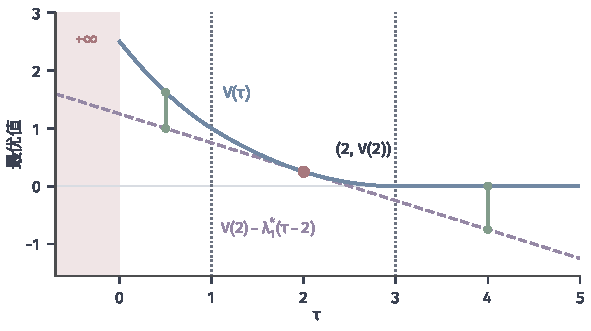
\includegraphics[width=100mm]{figures/05-optimization/06-constrained-optimization/matplotlib/sens-global-bound/figure.pdf}
 \caption{预算例的最优值函数（蓝线）和由$\tau=2$处乘子$\lambda_1^\star=1/2$给出的下界（紫色虚线）。红点是基准点，绿色线段是$\tau=0.5$和$\tau=4$处下界的余量，灰色点线标出活动约束改变的$\tau=1,3$。红色区域$\tau<0$不可行，$V=+\infty$。}
 \label{fig:sens-global-bound}
\end{BookInlineFigure}

\paragraph{去掉强对偶会怎样}
强对偶达到这个条件不能换成“存在KKT乘子”。考虑非凸问题
\[
 \min_{x\in\mathbb{R}}\ -x^2\quad\text{s.t.}\quad x-1\leq u,\ \ -x-1\leq0.
\]
基准问题$u=0$的可行集是$[-1,1]$，$f^\star=-1$，在$x=\pm1$取得。

在$x=1$处，平稳条件$-2x+\lambda_1=0$给出KKT乘子$\lambda_1=2$，第二条约束不起作用，$\lambda_2=0$。如果照搬式~\eqref{eq:sens-rhs-bound}，会得到$V(u)\geq-1-2u$。

直接计算最优值。$u>0$时可行集是$[-1,1+u]$，最小点在$x=1+u$。$-2\leq u\leq0$时，可行集右端点的绝对值不超过$1$，最小点在$x=-1$。所以
\[
 V(u)=\begin{cases}-1,&-2\leq u\leq0,\\-(1+u)^2,&u>0.\end{cases}
\]
$u>0$时，
\[
 V(u)-(-1-2u)=-u^2<0,
\]
下界不成立，见图~\ref{fig:sens-kkt-no-bound}。原因是这个问题的对偶函数对任何乘子都是$-\infty$，强对偶不成立。KKT乘子只承载局部信息，全局下界必须由对偶最优的乘子给出。

\begin{BookInlineFigure}
 \centering
 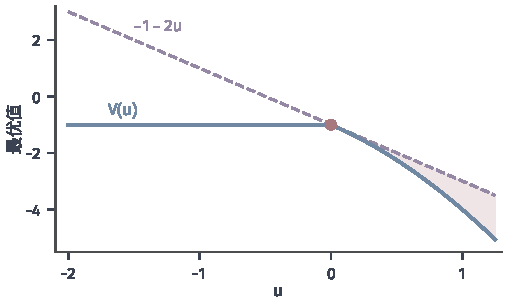
\includegraphics[width=86mm]{figures/05-optimization/06-constrained-optimization/matplotlib/sens-kkt-no-bound/figure.pdf}
 \caption{KKT乘子不给出全局下界的例子。蓝线是$\min-x^2$，$x-1\leq u$，$x\geq-1$的最优值$V(u)$，紫色虚线是用$x=1$处KKT乘子$2$写出的直线$-1-2u$，红色区域表示$u>0$时直线高于$V$。}
 \label{fig:sens-kkt-no-bound}
\end{BookInlineFigure}

非凸并不一定导致失败。对问题$\min-x^2$，$x^2-1\leq u$，取$\lambda=1$，Lagrange函数恒等于$-1$，所以$q(1)=-1=f^\star$。此时$V(u)=-1-u$（$u\geq-1$），下界恰好取等号。起决定作用的是零间隙，而不是凸性。

\subsection{乘子的边际解释}
\label{sec:sens-marginal}

下界只说明$V$不低于一条直线。什么时候这条直线就是$V$的切线，乘子就是最优值的真实变化率？本小节回答这个问题。

\paragraph{直线贴着曲线时}
一条直线处处不高于曲线，又在基准点与曲线相交。如果曲线在该点光滑，直线就没有选择，只能是切线。这正是图~\ref{fig:sens-global-bound}中红点处的情形。把这个几何观察写成定理：

\begin{theorem}[乘子是边际变化率]
\label{thm:sens-marginal}
在定理~\ref{thm:sens-rhs-bound}的条件下，进一步设$V$在$(\bm{0},\bm{0})$附近有限且在$(\bm{0},\bm{0})$可微，则
\begin{equation}
 \frac{\partial V}{\partial u_i}(\bm{0},\bm{0})=-\lambda_i^\star,
 \qquad
 \frac{\partial V}{\partial v_j}(\bm{0},\bm{0})=-\nu_j^\star.
 \label{eq:sens-marginal}
\end{equation}
\end{theorem}

\begin{proof}
定义函数
\[
 \varphi(\bm{u},\bm{v})=V(\bm{u},\bm{v})-f^\star+\langle\bm{\lambda}^\star,\bm{u}\rangle+\langle\bm{\nu}^\star,\bm{v}\rangle.
\]
式~\eqref{eq:sens-rhs-bound}说明$\varphi\geq0$，而$\varphi(\bm{0},\bm{0})=0$，所以原点是$\varphi$的极小点。原点是定义域的内点，$\varphi$在原点可微，它的梯度必须为零。写出这个梯度的各个分量，就是式~\eqref{eq:sens-marginal}。
\end{proof}

定理同时说明，只要$V$在基准点可微，满足条件的乘子就是唯一的，因为它们都等于$V$的梯度的相反数。

\paragraph{几何含义}
在预算例中，$-\nabla f(\bm{x}^\star)=\lambda_1^\star(1,1)$垂直于预算线。图~\ref{fig:sens-shadow-price-geometry}中，预算增加$\Delta\tau$时，预算线沿法向平移$\Delta\tau/\sqrt{2}$。目标沿法向的变化率是
\[
 \lVert\nabla f(\bm{x}^\star)\rVert_2=\lambda_1^\star\sqrt{2}.
\]
两者相乘，目标的一阶下降量是$\lambda_1^\star\Delta\tau$，这就是乘子作为\emph{影子价格}的含义：多一单位预算大约值$\lambda_1^\star$。没有起作用的约束乘子为零，放宽它们一阶没有价值。

\begin{BookInlineFigure}
 \centering
 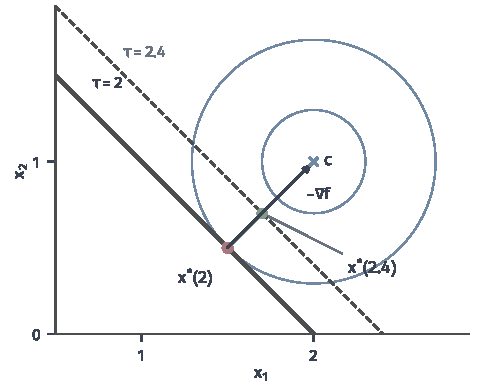
\includegraphics[width=84mm]{figures/05-optimization/06-constrained-optimization/matplotlib/sens-shadow-price-geometry/figure.pdf}
 \caption{预算线平移与乘子。深灰实线是$\tau=2$的预算线，虚线是$\tau=2.4$的预算线，蓝色圆是目标等高线。黑色箭头是$-\nabla f(\bm{x}^\star)=\lambda_1^\star(1,1)$，从红点指向理想点$\bm{c}$。绿色线段是最优解的移动。}
 \label{fig:sens-shadow-price-geometry}
\end{BookInlineFigure}

核对数值。$1<\tau<3$时，$V(\tau)=(3-\tau)^2/4$，这个公式将在第~\ref{sec:sens-active-change}节推出。于是$V'(2)=-1/2=-\lambda_1^\star$。取$\Delta\tau=0.4$，一阶估计是$0.25-0.2=0.05$，真实值$V(2.4)=0.09$。一阶估计恰好等于式~\eqref{eq:sens-budget-bound}的下界，真实值在它上方。

\paragraph{值函数不可微时}
可微性不是自动成立的。下面的引理不要求可微，并且给出了全局下界的完整刻画：所有能作全局下界斜率的向量，恰好就是全体最优乘子的相反数。

\begin{lemma}[下界斜率与最优乘子]
\label{lem:sens-support-multipliers}
设$f^\star$有限，$\bm{\lambda}\in\mathbb{R}^m$，$\bm{\nu}\in\mathbb{R}^p$，$f,g_i,h_j$定义在同一集合$\bm{D}$上，式~\eqref{eq:sens-rhs-value}及对偶函数中的$\bm{x}$都取遍$\bm{D}$。则下面两条等价：
\begin{enumerate}
 \item $\bm{\lambda}\geq\bm{0}$，且$q(\bm{\lambda},\bm{\nu})=f^\star$；
 \item 对所有$(\bm{u},\bm{v})$，都有
 \begin{equation}
  V(\bm{u},\bm{v})\geq f^\star-\langle\bm{\lambda},\bm{u}\rangle-\langle\bm{\nu},\bm{v}\rangle.
  \label{eq:sens-support}
 \end{equation}
\end{enumerate}
\end{lemma}

\begin{proof}
第一条推出第二条，这就是定理~\ref{thm:sens-rhs-bound}。下面从第二条出发。先证明$\lambda_i\geq0$。取$t>0$，令$\bm{u}=t\bm{e}_i$，$\bm{v}=\bm{0}$。放宽约束只会扩大可行集，所以$V(t\bm{e}_i,\bm{0})\leq f^\star$。结合式~\eqref{eq:sens-support}，得到
\[
 f^\star\geq V(t\bm{e}_i,\bm{0})\geq f^\star-t\lambda_i.
\]
所以$\lambda_i\geq0$。

再证明$q(\bm{\lambda},\bm{\nu})\geq f^\star$。任取$\bm{x}\in\bm{D}$，令$u_i=g_i(\bm{x})$，$v_j=h_j(\bm{x})$。这个$\bm{x}$是这组扰动问题的可行点，所以$f(\bm{x})\geq V(\bm{u},\bm{v})$。再由式~\eqref{eq:sens-support}，
\[
 f(\bm{x})\geq f^\star-\sum_i\lambda_ig_i(\bm{x})-\sum_j\nu_jh_j(\bm{x}).
\]

移项得到
\[
 \mathcal{L}(\bm{x},\bm{\lambda},\bm{\nu})\geq f^\star.
\]
对$\bm{x}$取下确界，得到$q(\bm{\lambda},\bm{\nu})\geq f^\star$。又由弱对偶$q(\bm{\lambda},\bm{\nu})\leq f^\star$，所以两者相等。
\end{proof}

当$f$与$g_i$是凸函数、$h_j$是仿射函数时，$V$是凸函数。取两组扰动及各自的近优可行点，它们的凸组合对扰动的相应凸组合仍可行，目标值不超过相应的凸组合，由此就得到$V$的凸性。

这时式~\eqref{eq:sens-support}正是第~\ref{chap:nonsmooth-composite-optimization}章次梯度的定义，引理说的就是$-(\bm{\lambda},\bm{\nu})$属于$V$在原点的次微分。若原点还是$V$的定义域的内点，$V$在方向$(\bm{u},\bm{v})$上的方向导数等于
\begin{equation}
 V'\bigl(\bm{0},\bm{0};\bm{u},\bm{v}\bigr)=\max_{(\bm{\lambda},\bm{\nu})\ \text{最优}}\bigl(-\langle\bm{\lambda},\bm{u}\rangle-\langle\bm{\nu},\bm{v}\rangle\bigr),
 \label{eq:sens-directional}
\end{equation}
其中最大值取遍全部最优乘子。这个等式的证明需要用到凸函数方向导数与次微分的对偶关系，篇幅较长，读者可查阅\scite{rockafellar1970convex}。它的含义是：每个方向上的真实变化率由“最不利”的乘子决定，单独一组乘子不能代表所有方向。

\paragraph{一个有折角的例子}
考虑一维问题
\[
 \min_{x\in\mathbb{R}}\ -x\quad\text{s.t.}\quad x-1\leq u,\ \ x-1\leq0.
\]
两条约束在$u=0$时完全相同，$x^\star=1$，$f^\star=-1$。Lagrange函数是
\[
 \mathcal{L}(x,\bm{\lambda})=(-1+\lambda_1+\lambda_2)x-\lambda_1-\lambda_2.
\]

$\lambda_1+\lambda_2\neq1$时它对$x$无下界。$\lambda_1+\lambda_2=1$时它恒等于$-1$。所以最优乘子集合是线段$\{\bm{\lambda}\geq\bm{0}:\lambda_1+\lambda_2=1\}$，乘子不唯一。

右端扰动的最优值可以直接写出。$u\geq0$时第二条约束决定解，$x=1$；$u<0$时第一条约束决定解，$x=1+u$。所以
\[
 V(u)=\max\{-1-u,\ -1\}.
\]

$V$在$u=0$处有折角，左导数是$-1$，右导数是$0$。图~\ref{fig:sens-subgrad-kink}(a)中斜率在$[-1,0]$内的每条直线都是全局下界，它们恰好对应(b)中线段上的每个乘子。

由式~\eqref{eq:sens-directional}，向右的方向导数$V'(0;1)=\max(-\lambda_1)=0$，由$\lambda_1=0$取到。向左的方向导数$V'(0;-1)=\max\lambda_1=1$，由$\lambda_1=1$取到。求解器如果返回对称的乘子$(1/2,1/2)$，那么$-1/2$只是一个合法的下界斜率，不是任何方向上的导数。

\begin{BookInlineFigure}
 \centering
 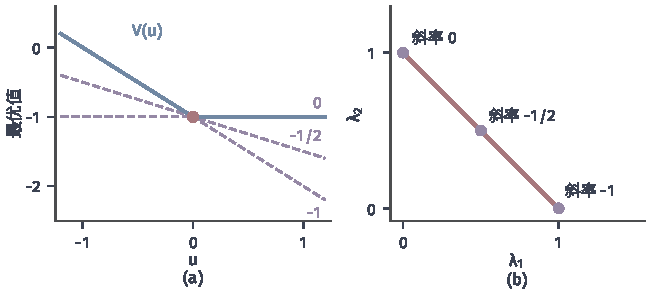
\includegraphics[width=112mm]{figures/05-optimization/06-constrained-optimization/matplotlib/sens-subgrad-kink/figure.pdf}
 \caption{乘子不唯一时的值函数。(a)~蓝线是$V(u)=\max\{-1-u,-1\}$，紫色虚线是斜率$0,-1/2,-1$的全局下界，它们都穿过红点。(b)~红色线段是全体最优乘子，紫色点是图(a)三条直线对应的乘子。}
 \label{fig:sens-subgrad-kink}
\end{BookInlineFigure}

表~\ref{tab:sens-three-slopes}比较本节出现的三个量。

\begin{BookInlineTable}
 \centering
 \begin{tabular}{lll}
  \toprule
  对象 & 成立条件 & 范围\\
  \midrule
  下界斜率$-\bm{\lambda}^\star$ & 零间隙且乘子达到 & 全局，单侧\\
  实际导数$-\bm{\lambda}^\star$ & 另加$V$在基准点可微 & 局部，一阶\\
  方向导数 & 凸问题、基准点在定义域内部 & 局部，沿给定方向\\
  \bottomrule
 \end{tabular}
 \caption{约束右端扰动下的三个量。下界斜率来自任何一组最优乘子，实际导数要求$V$可微，方向导数要在全体最优乘子上取最大值。}
 \label{tab:sens-three-slopes}
\end{BookInlineTable}

\subsection{目标参数的包络关系}
\label{sec:sens-envelope}

现在让目标函数含参数，可行集固定。最优解随参数移动，所以最优值的变化似乎有两个来源：目标本身变了，最优点也动了。本小节的结论是，一阶意义下第二个来源不起作用。

\paragraph{谷底的一阶平坦}
站在谷底，向任何方向走一小步，高度的一阶变化都是零。最优解被参数推着移动一小段，走的正是这样的一小步，所以高度的变化几乎全部来自地形本身的改变。这是整个包络关系的直观基础。

在边界上情况稍有不同：梯度不必为零，因为有约束挡住。但如果解沿着边界来回移动，它向两个相反的方向都是可行的，梯度只能与这个移动方向垂直。

\begin{theorem}[包络关系]
\label{thm:sens-envelope}
设$\bm{C}\subseteq\mathbb{R}^n$固定，$f$在$(\bm{x}_0,\bm{\theta}_0)$的邻域内连续可微。设映射$\bm{x}(\cdot)$定义在$\bm{\theta}_0$的邻域上，取值于$\bm{C}$，在$\bm{\theta}_0$处可微，$\bm{x}(\bm{\theta}_0)=\bm{x}_0$，且$\bm{x}_0$是$f(\cdot,\bm{\theta}_0)$在$\bm{C}$上的局部极小点。记$v$为式~\eqref{eq:sens-branch-value}定义的分支值，则
\begin{equation}
 \nabla v(\bm{\theta}_0)=\nabla_{\bm{\theta}}f(\bm{x}_0,\bm{\theta}_0).
 \label{eq:sens-envelope}
\end{equation}
\end{theorem}

\begin{proof}
记$\bm{D}_{\bm{x}}\in\mathbb{R}^{n\times q}$是$\bm{x}(\cdot)$在$\bm{\theta}_0$的Jacobian矩阵。由链式法则，
\[
 \nabla v(\bm{\theta}_0)=\nabla_{\bm{\theta}}f(\bm{x}_0,\bm{\theta}_0)+\bm{D}_{\bm{x}}^{\top}\nabla_{\bm{x}}f(\bm{x}_0,\bm{\theta}_0).
\]
只需证明第二项为零。任取方向$\bm{d}\in\mathbb{R}^q$，令
\[
 \psi(t)=f\bigl(\bm{x}(\bm{\theta}_0+t\bm{d}),\bm{\theta}_0\bigr).
\]

注意$\psi$里的参数固定在$\bm{\theta}_0$。$\lvert t\rvert$很小时，$\bm{x}(\bm{\theta}_0+t\bm{d})$属于$\bm{C}$且靠近$\bm{x}_0$，所以$\psi(t)\geq\psi(0)$。$t=0$是$\psi$的内部极小点，$\psi'(0)=0$，也就是
\[
 \bigl\langle\nabla_{\bm{x}}f(\bm{x}_0,\bm{\theta}_0),\ \bm{D}_{\bm{x}}\bm{d}\bigr\rangle=0.
\]
$\bm{d}$是任意的，所以
\[
 \bm{D}_{\bm{x}}^{\top}\nabla_{\bm{x}}f(\bm{x}_0,\bm{\theta}_0)=\bm{0}.
\]
\end{proof}

结论说的是分支上的值$v$，而不是全局最优值$V$。条件里最关键的是$\bm{C}$固定：这样分支上的点对基准问题仍是可行的，才能用基准点的局部极小性。约束也含参数的情形放在第~\ref{sec:sens-general-constraints}节。

\paragraph{预算例：理想点移动}
把理想点改成$(2+\theta,1)$，预算固定为$\tau=2$，目标是
\[
 f(\bm{x},\theta)=\frac12(x_1-2-\theta)^2+\frac12(x_2-1)^2.
\]
$\lvert\theta\rvert<1$时只有预算起作用。平稳条件是$x_1-2-\theta+\lambda=0$、$x_2-1+\lambda=0$，与$x_1+x_2=2$联立，得到
\[
 \lambda=\frac{1+\theta}{2},\qquad
 x_1(\theta)=\frac32+\frac{\theta}{2},\qquad
 x_2(\theta)=\frac12-\frac{\theta}{2}.
\]

分支上的值是$v(\theta)=\lambda^2=(1+\theta)^2/4$，直接求导得到$v'(\theta)=(1+\theta)/2$。用包络关系，只需对目标中显含的$\theta$求偏导：
\[
 \frac{\partial f}{\partial\theta}=2+\theta-x_1=\frac{1+\theta}{2}.
\]
两个结果一致。解的移动方向是$\bm{x}'(\theta)=(1/2,-1/2)$，$\nabla_{\bm{x}}f=-\lambda(1,1)$，两者的内积确实为零。图~\ref{fig:sens-envelope}(a)显示，解沿预算线滑动，而负梯度垂直于这条线。

\paragraph{为什么叫包络}
把决策$\hat{\bm{x}}$固定，$\theta\mapsto f(\hat{\bm{x}},\theta)$就是一条曲线。每个固定的决策对应一条这样的曲线，它们都在$v(\theta)$上方，因为固定决策不会比最优决策好。图~\ref{fig:sens-envelope}(b)中$v$是这族曲线的下边缘，称为它们的\emph{包络}，式~\eqref{eq:sens-envelope}因此称为\term{包络定理}（envelope theorem）。

曲线在切点处与$v$相切。切点处的斜率既是这条固定决策曲线的斜率，也是$v$的斜率，这正是“只对显含的$\theta$求导”的图形含义。

\begin{BookInlineFigure}
 \centering
 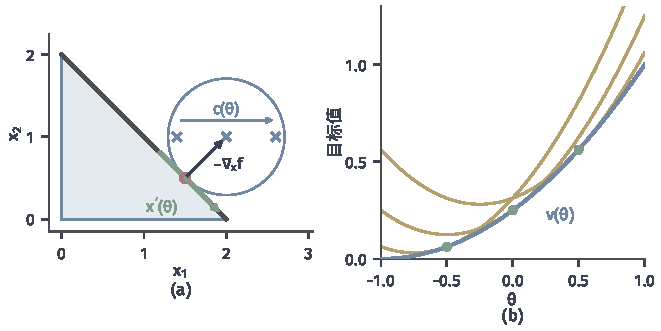
\includegraphics[width=112mm]{figures/05-optimization/06-constrained-optimization/matplotlib/sens-envelope/figure.pdf}
 \caption{包络关系。(a)~$\tau=2$的可行集上，理想点沿蓝色箭头移动（蓝色叉是$\theta=-0.6,0,0.6$），最优解沿绿色线段滑动。红点是$\theta=0$的解，黑色箭头是负梯度，绿色箭头是解的移动方向，两者垂直。(b)~黄线是把决策固定在$\theta=-0.5,0,0.5$的最优解上得到的目标值，蓝线$v(\theta)$是它们的下边缘，绿点是切点。}
 \label{fig:sens-envelope}
\end{BookInlineFigure}

\paragraph{没有可微分支时}
定理~\ref{thm:sens-envelope}需要一条可微的解分支。若最优解不唯一，或最优解随参数跳动，这样的分支就没有了。但只要可行集紧，全局最优值的方向导数仍然有公式，这就是Danskin型结果。

\begin{theorem}[Danskin型结果]
\label{thm:sens-danskin}
设$\bm{C}\subseteq\mathbb{R}^n$非空且紧，$\bm{\Theta}\subseteq\mathbb{R}^q$开，$f$在$\bm{C}\times\bm{\Theta}$上连续，关于$\bm{\theta}$的梯度$\nabla_{\bm{\theta}}f$存在且在$\bm{C}\times\bm{\Theta}$上连续。记$V$为式~\eqref{eq:sens-value}在$\bm{C}(\bm{\theta})\equiv\bm{C}$时的最优值函数，则对每个$\bm{\theta}\in\bm{\Theta}$与方向$\bm{d}$，
\begin{equation}
 V'(\bm{\theta};\bm{d})=\min_{\bm{x}\in\bm{S}(\bm{\theta})}\bigl\langle\nabla_{\bm{\theta}}f(\bm{x},\bm{\theta}),\bm{d}\bigr\rangle.
 \label{eq:sens-danskin}
\end{equation}
若$\bm{S}(\bm{\theta})=\{\bm{x}^\star\}$只有一个点，则$V$在$\bm{\theta}$可微，且
\begin{equation}
 \nabla V(\bm{\theta})=\nabla_{\bm{\theta}}f(\bm{x}^\star,\bm{\theta}).
 \label{eq:sens-danskin-gradient}
\end{equation}
\end{theorem}

\begin{proof}
$\bm{S}(\bm{\theta})$是紧集$\bm{C}$的闭子集，所以式~\eqref{eq:sens-danskin}的最小值可以取到。下面从两个方向夹逼。

先证上界。任取$\bm{x}\in\bm{S}(\bm{\theta})$和$t>0$。$\bm{x}$对$\bm{\theta}+t\bm{d}$仍可行，而且在$\bm{\theta}$处最优，所以
\[
 V(\bm{\theta}+t\bm{d})\leq f(\bm{x},\bm{\theta}+t\bm{d}),\qquad V(\bm{\theta})=f(\bm{x},\bm{\theta}).
\]
由一元中值定理，存在$\xi\in(0,1)$，使
\[
 \frac{V(\bm{\theta}+t\bm{d})-V(\bm{\theta})}{t}\leq\bigl\langle\nabla_{\bm{\theta}}f(\bm{x},\bm{\theta}+\xi t\bm{d}),\bm{d}\bigr\rangle.
\]
令$t\downarrow0$，由梯度的连续性，上极限不超过$\langle\nabla_{\bm{\theta}}f(\bm{x},\bm{\theta}),\bm{d}\rangle$。再对$\bm{x}\in\bm{S}(\bm{\theta})$取最小，就得到上界。

再证下界。取$t_k\downarrow0$，使差商趋于它的下极限，并取$\bm{x}_k\in\bm{S}(\bm{\theta}+t_k\bm{d})$。$\bm{C}$是紧集，可以取子列使$\bm{x}_k\to\bar{\bm{x}}\in\bm{C}$。对任意$\bm{y}\in\bm{C}$，$\bm{x}_k$的最优性给出
\[
 f(\bm{x}_k,\bm{\theta}+t_k\bm{d})\leq f(\bm{y},\bm{\theta}+t_k\bm{d}).
\]
令$k\to\infty$并用$f$的连续性，可知$\bar{\bm{x}}$在参数$\bm{\theta}$下的目标值不超过任何$\bm{y}\in\bm{C}$的目标值，所以$\bar{\bm{x}}\in\bm{S}(\bm{\theta})$。

此外，$\bm{x}_k$是基准问题的可行点，又在$\bm{\theta}+t_k\bm{d}$处最优，所以
\[
 V(\bm{\theta})\leq f(\bm{x}_k,\bm{\theta}),\qquad V(\bm{\theta}+t_k\bm{d})=f(\bm{x}_k,\bm{\theta}+t_k\bm{d}).
\]
再用一次中值定理，存在$\xi_k\in(0,1)$，使
\[
 \frac{V(\bm{\theta}+t_k\bm{d})-V(\bm{\theta})}{t_k}\geq\bigl\langle\nabla_{\bm{\theta}}f(\bm{x}_k,\bm{\theta}+\xi_kt_k\bm{d}),\bm{d}\bigr\rangle.
\]
令$k\to\infty$，下极限不小于$\langle\nabla_{\bm{\theta}}f(\bar{\bm{x}},\bm{\theta}),\bm{d}\rangle$，它又不小于式~\eqref{eq:sens-danskin}的右端。上下界合起来，方向导数存在并等于右端。

只有一个解时，把上面两步中的$t\bm{d}$换成趋于零的向量$\bm{\delta}$。上界一步给出
\[
 V(\bm{\theta}+\bm{\delta})-V(\bm{\theta})\leq\langle\nabla_{\bm{\theta}}f(\bm{x}^\star,\bm{\theta}),\bm{\delta}\rangle+o(\lVert\bm{\delta}\rVert_2).
\]
下界一步中$\bm{x}_{\bm{\delta}}\to\bm{x}^\star$，因为任何极限点都属于单点集$\bm{S}(\bm{\theta})$，于是相同的表达式也是下界。所以$V$可微。
\end{proof}

式~\eqref{eq:sens-danskin}取的是最小值，这与目标是最小化相对应。直观上，参数沿$\bm{d}$变化时，全部最优解处在同一起跑线上，下一时刻仍然留在最优的，是在方向$\bm{d}$上目标增长最慢的那一个。

\paragraph{条件的作用：多解时的方向导数}
考虑线性目标$f(\bm{x},p)=-px_1-x_2$，可行集是$\tau=2$的三角形。$p>1$时最优点是$(2,0)$，$p<1$时最优点是$(0,2)$，$p=1$时整条预算线都是最优解，见图~\ref{fig:sens-danskin-edge}。最优值是
\[
 V(p)=-2\max\{p,1\}.
\]

在$p=1$处，$\partial f/\partial p=-x_1$。式~\eqref{eq:sens-danskin}给出
\[
 V'(1;1)=\min_{\bm{x}\in\bm{S}(1)}(-x_1)=-2,\qquad
 V'(1;-1)=\min_{\bm{x}\in\bm{S}(1)}x_1=0.
\]
第一个由顶点$(2,0)$取到，第二个由顶点$(0,2)$取到，与图中两段的斜率一致。

\begin{BookInlineFigure}
 \centering
 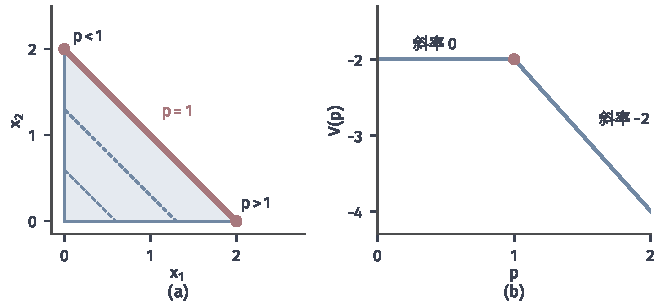
\includegraphics[width=112mm]{figures/05-optimization/06-constrained-optimization/matplotlib/sens-danskin-edge/figure.pdf}
 \caption{线性目标$-px_1-x_2$在三角形$x_1+x_2\leq2$，$\bm{x}\geq\bm{0}$上的最优解。(a)~$p=1$时蓝色虚线的等值线平行于预算线，红色粗线上的点都最优；$p>1$或$p<1$时解是相应的红色顶点。(b)~最优值$V(p)=-2\max\{p,1\}$在$p=1$有折角。}
 \label{fig:sens-danskin-edge}
\end{BookInlineFigure}

紧性不能随意去掉。第~\ref{sec:sens-problems}节的$f(x,\theta)=e^x-\theta x$在$\theta=0$处没有最优解，式~\eqref{eq:sens-danskin}的右端失去意义。实际上$\theta>0$时$V(\theta)=\theta-\theta\ln\theta$，所以
\[
 \frac{V(\theta)-V(0)}{\theta}=1-\ln\theta\to+\infty\quad(\theta\downarrow0),
\]
$V$在$\theta=0$处的右导数不是有限数。

\subsection{一般含参约束}
\label{sec:sens-general-constraints}

现在目标和约束都含参数。可行集随参数移动，上一小节的证明不能直接用，因为分支上的点对基准问题已经不可行。本小节说明，对沿分支的值求导时，Lagrange函数吸收了约束移动的贡献。

\paragraph{从目标到Lagrange函数}
考虑一族问题
\begin{equation}
 \min_{\bm{x}}\ f(\bm{x},\bm{\theta})\quad
 \text{s.t.}\quad g_i(\bm{x},\bm{\theta})\leq0,\ \ h_j(\bm{x},\bm{\theta})=0,
 \label{eq:sens-general-problem}
\end{equation}
其Lagrange函数$\mathcal{L}(\bm{x},\bm{\lambda},\bm{\nu},\bm{\theta})$也含参数。下面的定理假设已经有一条KKT点分支，并且起作用的约束保持起作用。这条分支从何而来，由第~\ref{sec:sens-solution}节回答。

\begin{theorem}[分支值对参数的导数]
\label{thm:sens-general-branch}
设$f,g_i,h_j$在$(\bm{x}_0,\bm{\theta}_0)$的邻域内连续可微。设映射$\bm{x}(\cdot)$在$\bm{\theta}_0$的邻域上满足$\bm{x}(\bm{\theta}_0)=\bm{x}_0$，在$\bm{\theta}_0$可微，$(\bm{x}_0,\bm{\lambda}_0,\bm{\nu}_0)$在$\bm{\theta}_0$处满足平稳条件，且沿分支恒有
\begin{equation}
 g_i(\bm{x}(\bm{\theta}),\bm{\theta})=0\ \ (\lambda_{0,i}>0),\qquad
 h_j(\bm{x}(\bm{\theta}),\bm{\theta})=0.
 \label{eq:sens-active-held}
\end{equation}
记$v$为式~\eqref{eq:sens-branch-value}定义的分支值，则
\begin{equation}
 \nabla v(\bm{\theta}_0)=\nabla_{\bm{\theta}}\mathcal{L}(\bm{x}_0,\bm{\lambda}_0,\bm{\nu}_0,\bm{\theta}_0).
 \label{eq:sens-general-gradient}
\end{equation}
\end{theorem}

\begin{proof}
下面所有函数都在$(\bm{x}_0,\bm{\theta}_0)$取值，$\bm{D}_{\bm{x}}$是分支的Jacobian矩阵。由链式法则，
\[
 \nabla v=\nabla_{\bm{\theta}}f+\bm{D}_{\bm{x}}^{\top}\nabla_{\bm{x}}f.
\]
用平稳条件替换$\nabla_{\bm{x}}f$，乘子为零的项自动消失：
\[
 \bm{D}_{\bm{x}}^{\top}\nabla_{\bm{x}}f=-\sum_{i}\lambda_{0,i}\bm{D}_{\bm{x}}^{\top}\nabla_{\bm{x}}g_i-\sum_j\nu_{0,j}\bm{D}_{\bm{x}}^{\top}\nabla_{\bm{x}}h_j.
\]

对恒等式$g_i(\bm{x}(\bm{\theta}),\bm{\theta})=0$求导，得到
\[
 \bm{D}_{\bm{x}}^{\top}\nabla_{\bm{x}}g_i+\nabla_{\bm{\theta}}g_i=\bm{0}.
\]
等式约束同样如此。代回上一式，得到
\[
 \bm{D}_{\bm{x}}^{\top}\nabla_{\bm{x}}f=\sum_i\lambda_{0,i}\nabla_{\bm{\theta}}g_i+\sum_j\nu_{0,j}\nabla_{\bm{\theta}}h_j.
\]
加上$\nabla_{\bm{\theta}}f$，右端就是$\nabla_{\bm{\theta}}\mathcal{L}$。
\end{proof}

式~\eqref{eq:sens-general-gradient}包含两部分贡献。$\nabla_{\bm{\theta}}f$是目标本身的变化，$\sum\lambda_i\nabla_{\bm{\theta}}g_i$是约束移动造成的变化，乘子把约束的移动折算成目标的变化。若约束不含参数，第二部分为零，回到包络关系。若$g_1=x_1+x_2-\tau$，则$\partial g_1/\partial\tau=-1$，式~\eqref{eq:sens-general-gradient}给出$v'(\tau)=-\lambda_1$，回到边际解释。

\paragraph{一个目标与约束同时含参的例子}
让参数$\theta$同时影响目标和预算的价格：
\[
 \min_{\bm{x}}\ \frac12(x_1-1-\theta)^2+\frac12(x_2-1)^2
 \quad\text{s.t.}\quad \theta x_1+x_2-2\leq0.
\]
$\theta=1$时它就是$\tau=2$的预算例。$\theta$变大时，第一种投入的单价上涨，预算线绕$(0,2)$转动，理想点也同时右移，见图~\ref{fig:sens-moving-constraint}。

\begin{BookInlineFigure}
 \centering
 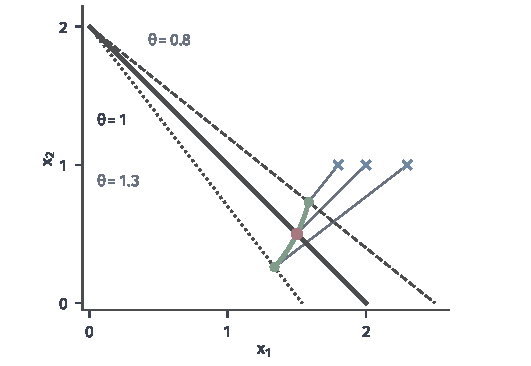
\includegraphics[width=90mm]{figures/05-optimization/06-constrained-optimization/matplotlib/sens-moving-constraint/figure.pdf}
 \caption{目标与约束同时含参。三条深灰线是$\theta=0.8,1,1.3$的预算线$\theta x_1+x_2=2$，蓝色叉是相应的理想点$(1+\theta,1)$，细灰线连接理想点和最优解。绿色曲线是最优解随$\theta$的路径，红点是$\theta=1$的解。}
 \label{fig:sens-moving-constraint}
\end{BookInlineFigure}

预算约束起作用时，平稳条件是$x_1-1-\theta+\lambda\theta=0$、$x_2-1+\lambda=0$。把$x_1=1+\theta-\lambda\theta$与$x_2=1-\lambda$代入$\theta x_1+x_2=2$，解出
\[
 \lambda(\theta)=\frac{\theta^2+\theta-1}{1+\theta^2}.
\]
$\theta=1$时$\lambda=1/2$，$\bm{x}=(3/2,1/2)$。

用式~\eqref{eq:sens-general-gradient}，目标与约束的偏导数分别是
\[
 \frac{\partial f}{\partial\theta}=-(x_1-1-\theta)=\lambda\theta=\frac12,
 \qquad
 \lambda\frac{\partial g}{\partial\theta}=\lambda x_1=\frac34.
\]
相加得到$v'(1)=5/4$。目标的直接变化贡献$1/2$，价格上涨使约束收紧，贡献$3/4$。

直接核对：把解代入目标，得到$v(\theta)=\tfrac12\lambda^2(1+\theta^2)$，即
\[
 v(\theta)=\frac{(\theta^2+\theta-1)^2}{2(1+\theta^2)}.
\]
在$\theta=1$处求导，分子$N=\theta^2+\theta-1$满足$N=1$，$N'=3$，分母$D=1+\theta^2$满足$D=2$，$D'=2$，所以
\[
 v'(1)=\frac{NN'}{D}-\frac{N^2D'}{2D^2}=\frac32-\frac14=\frac54.
\]
两个结果一致。式~\eqref{eq:sens-general-gradient}不需要先解出分支，只需要基准点的$\bm{x}$和乘子。
